\newpage 

\subsection{Use case diagram}
\label{subsec:useCaseDiagram}
Figur \ref{fig:UCD} viser de identificerede use cases.
\vspace{-10pt}
%Usecase diagram indføres i følgende 5 linjer, derefter starter UC 1
\begin{figure}[H]
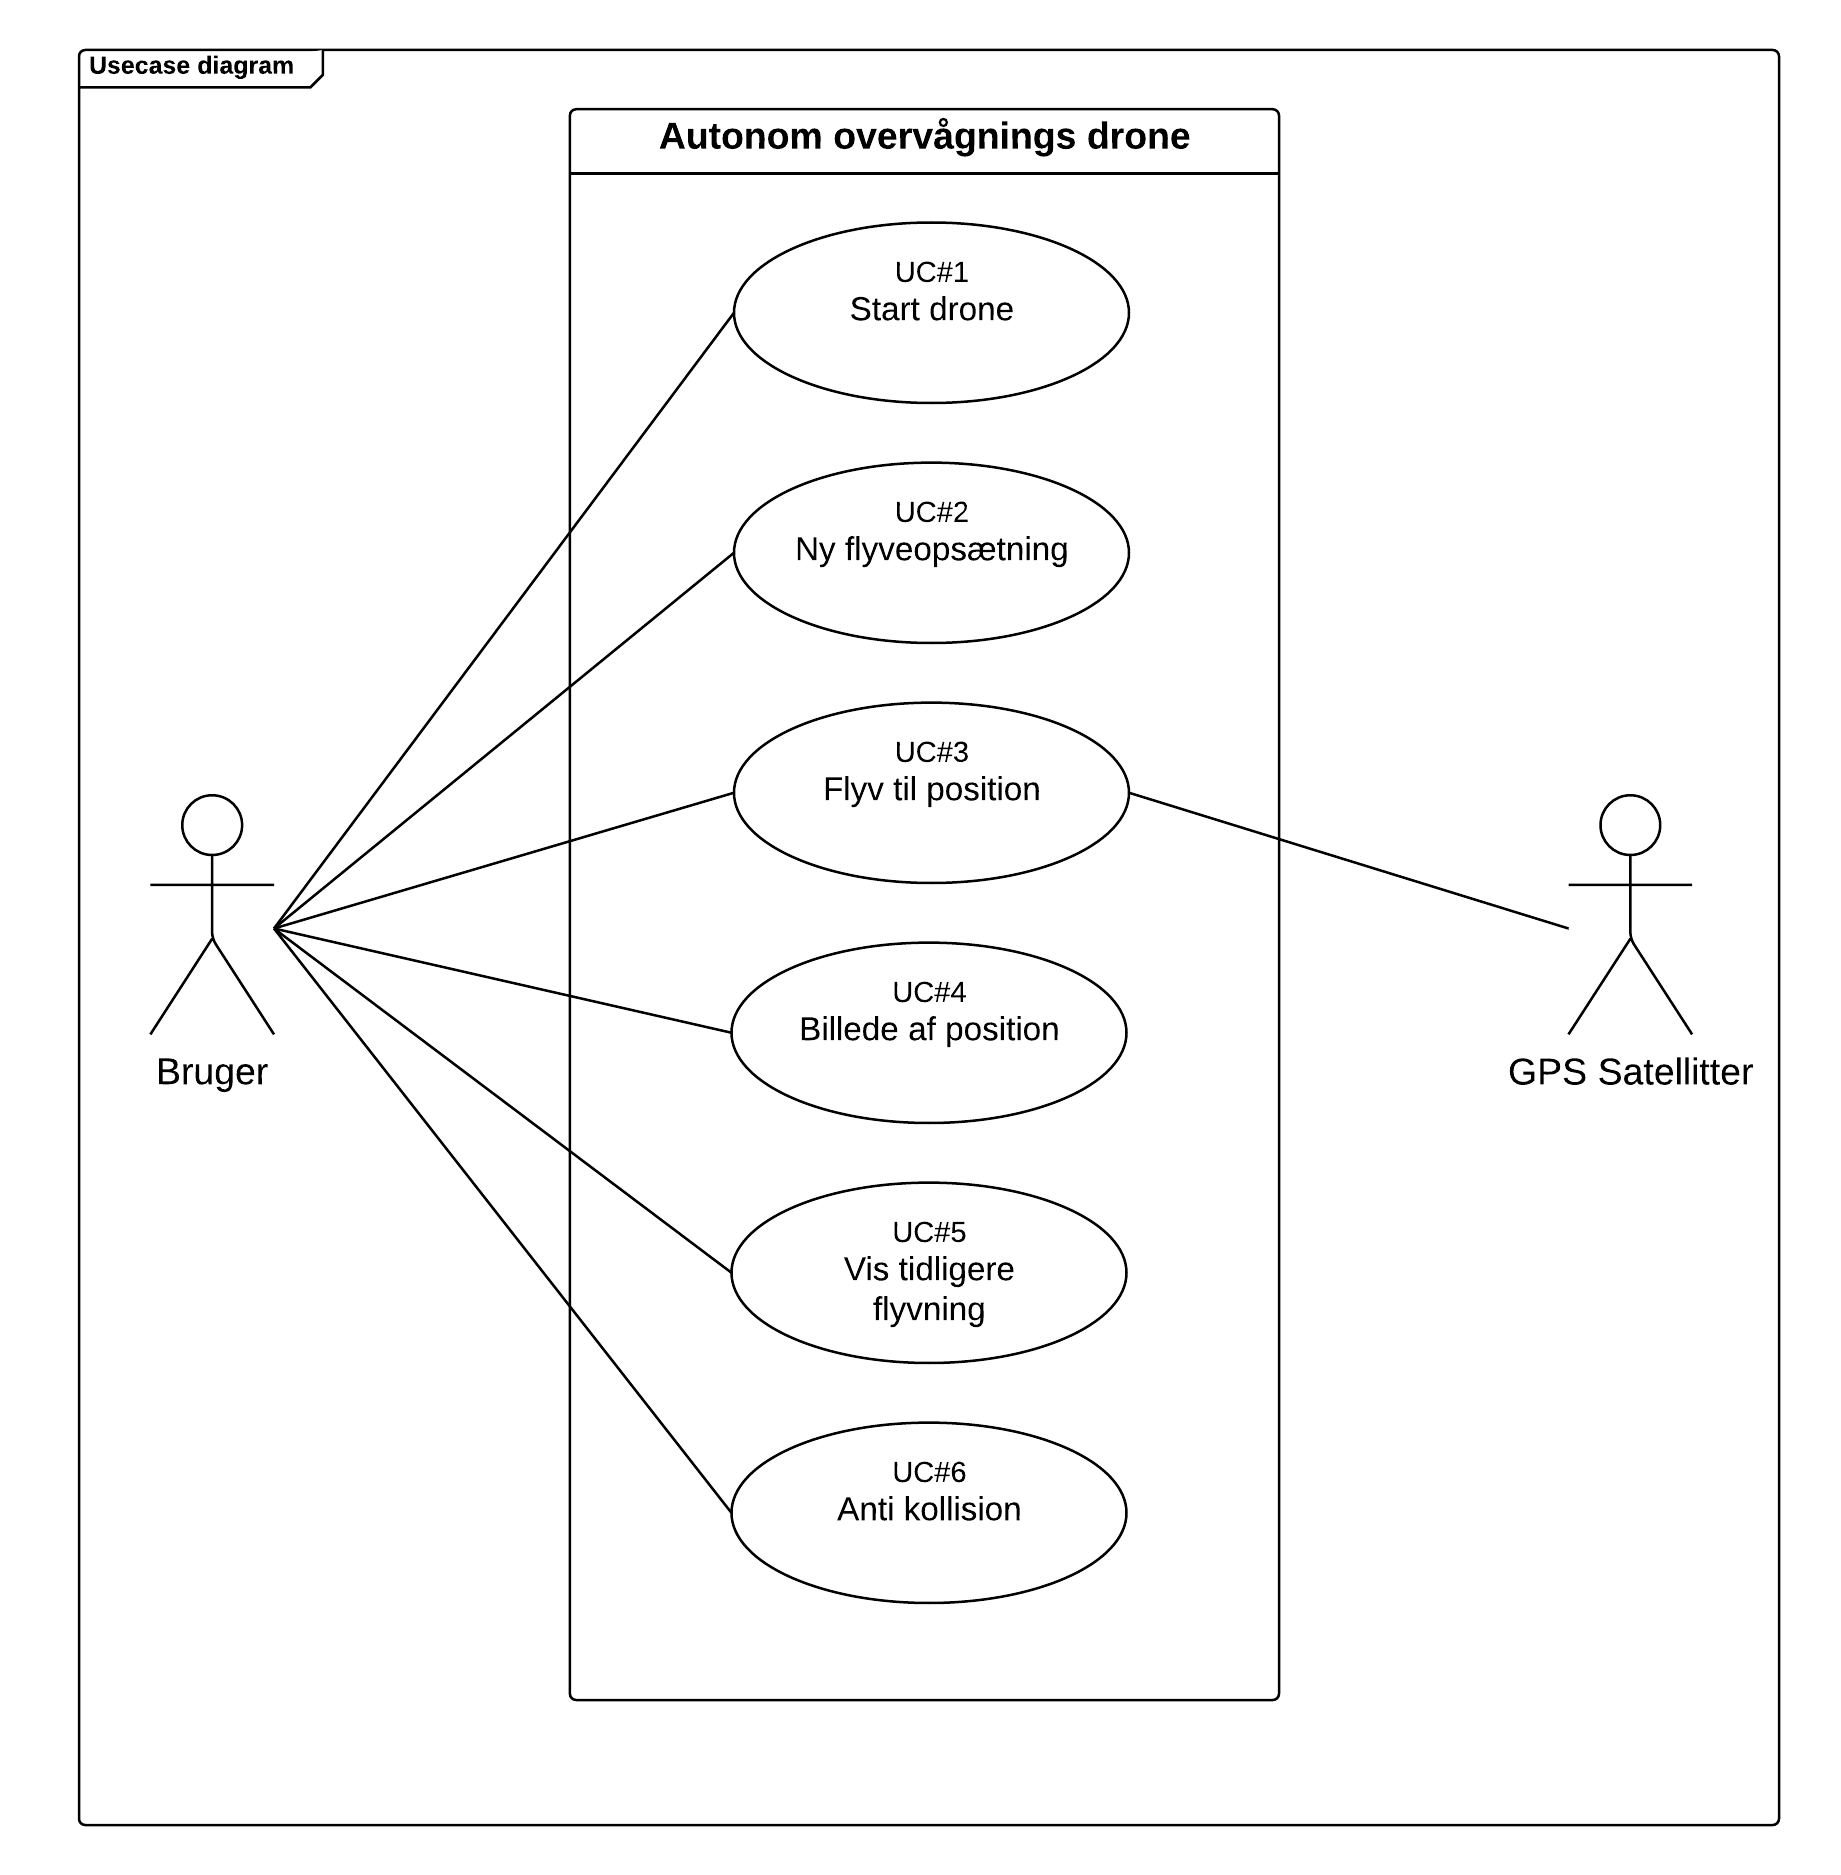
\includegraphics[width=1\textwidth]{Billeder/Use_case_diagram.png}
\vspace{-30pt}
\caption{Use case diagram}
\label{fig:UCD}
\end{figure}



\subsection{Udviklingsforløb}

For at tydeliggøre hvordan udviklingsforløbet  

\textbf{Iteration 1:}


\textbf{Iteration 2:}

\textbf{Iteration 3:}

\textbf{Iteration 4:}